\documentclass[a4paper,12pt]{report}
\usepackage[spanish,mexico]{babel}
\usepackage[utf8]{inputenc}
\usepackage[T1]{fontenc}
\usepackage{amsmath}
\usepackage{amssymb}
\usepackage{wasysym}
\usepackage[dvipsnames,pdftex]{color}
\usepackage[x11names]{xcolor}
\usepackage{tikz, tkz-euclide}
\usepackage[american]{circuitikz}
\usepackage{siunitx}
\usetikzlibrary{arrows}
\usepackage[colorinlistoftodos]{todonotes}
%\usepackage[left=2cm,right=1.5cm,top=1cm,bottom=1cm]{geometry}
%\usepackage{helvet}
%\renewcommand{\familydefault}{\sfdefault}
\setlength{\oddsidemargin}{0in}
\usepackage{geometry}
\geometry{a4paper, total = {180mm,270mm},
			left = 25mm, top = 20mm,
            right=15mm,bottom=20mm,%
            footskip=10mm}
\usepackage{float} 
% \setlength{\topmargin}{0in}
% \setlength{\voffset}{-0.5in}
% \setlength{\hoffset}{0.3in}
% \setlength{\textheight}{700pt}
% \setlength{\textwidth}{440pt}
% \setlength{\topskip}{0in}
% \setlength{\parskip}{2ex}
 \renewcommand{\baselinestretch}{1.5}
\usepackage{diagbox}
\usepackage{array}
\usepackage{listings}
\usepackage{caption}
%%% comandos definidos por el usuario
\begin{document}
\setcounter{page}{1}
\pagenumbering{roman}
\thispagestyle{empty}
\begin{center}
{\huge UNIVERSIDAD NACIONAL DE INGENIERÍA}\\[0.9cm]
{\Large FACULTAD DE INGENIERÍA MECÁNICA}\\[0.6in]
\end{center}
\begin{figure}[h]
\begin{center}

\includegraphics[scale=0.33]{logoUNI.png}
\vspace{0cm}
\end{center}
\end{figure}
\vspace{0.5cm}
\begin{center}
INFORME DE LABORATORIO\\
LABORATORIO DE CIRCUITOS ELÉCTRICOS\\[5mm]
{\large LEYES DE KIRCHHOFF Y RECONOCIMIENTO DE EQUIPOS}\\[10mm]
\vfill
LIMA - PERÚ \hfill SEPTIEMBRE 2019
\end{center}
\newpage
\thispagestyle{empty}
\begin{center}
{\Huge LEYES DE KIRCHHOFF Y RECONOCIMIENTO DE EQUIPOS}\\[0.7cm]
\small ENTREGADO:\\[0.05cm]
\small 11 SEPTIEMBRE 2019\\[1.2cm]
\end{center}
\begin{flushleft}
{\large ALUMNOS:}\\[2cm]
\end{flushleft}
\begin{tabular}{c@{\hspace{0.5in}}c}
\rule[1pt]{2.6in}{1pt}&\rule[1pt]{2.6in}{1pt}\\
Huaroto Villavicencio Josué, 20174070I & Landeo Sosa Bruno, 20172024J\\[2.5cm]
%\rule[1pt]{2.6in}{1pt}&\rule[1pt]{2.6in}{1pt}\\
%Perez La Rosa Fabrizio, 20170234G & Seclén Yberos Carlos, 20174137F\\[2.5cm]
\rule[1pt]{2.6in}{1pt}&\rule[1pt]{2.6in}{1pt}\\
Quesquén Vitor Angel, 20170270C & Sotelo Cavero Sergio, 20172125K\\[2.5cm]
\end{tabular}
%\begin{center}
%\begin{tabular}{c@{\hspace{0.5in}}c}
%\rule[1pt]{3.14in}{1pt}\\
%Sotelo Cavero Sergio, 20172125K% & Nombre 5, 2017 \\[1.5cm]
%\end{tabular}
%\end{center}
%\begin{center}
%\begin{tabular}{c@{\hspace{0.6in}}c}
%\rule[1pt]{3.14in}{1pt}\\
%Huaroto Villavicencio Josué, 20174070I \\[2cm]
%\rule[1pt]{3.14in}{1pt}\\
%Landeo Sosa Bruno, 20174070I \\[2cm]
%\rule[1pt]{3.14in}{1pt}\\
%Quesquén Vitor Angel, 20172125K \\[2cm]
%\rule[1pt]{3.14in}{1pt}\\
%Sotelo Cavero Sergio, 20172125K \\[2cm]
%\end{tabular}
%\end{center}
%\begin{center}
%\begin{tabular}{c}
%\rule[1pt]{3.14in}{1pt}\\
%Huaroto Villavicencio Josué, 20174070I \\[2.5cm]
%\end{tabular}
%\end{center}

%\rule[1pt]{3.14in}{1pt}\\
%Maguiña Amaya Wladimir, 20172019F \\[3cm]
%\rule[1pt]{3.14in}{1pt}\\
%Luis Sosa Jose, 19774147I \\[3cm]
%\rule[1pt]{3.14in}{1pt}\\
%Sotelo Cavero Sergio, 20172125K
%\end{tabular}
%\end{center}
%\\[0.7cm]
{\large PROFESOR:} \\[2cm]
\begin{center}
\begin{tabular}{c}
\rule[3pt]{4.8in}{1pt}\\[1pt]
ING. SINCHI YUPANQUI, FRANCISCO 
\end{tabular}
\end{center}
\vfill
%\newpage
%\begin{center}
%{\Large \bf{RESUMEN}}
%\end{center}
\newpage
\tableofcontents
\listoffigures
\addcontentsline{toc}{chapter}{Índice de figuras}
\newpage
\pagenumbering{arabic} %%% esto es para regresar el modo de numeración a numeración arábiga
\setcounter{page}{1}  %%% empezamos en página 1
%\part{Introducción}
\part{Introducción}
\chapter{Objetivos}
\begin{enumerate}
\item Familiarizarse con el manejo de los instrumentos del laboratorio.
\item Tomar en consideración las medidas de seguridad indicadas para la realización de un buen trabajo en el laboratorio.
\item Verificar experimentalmente las leyes de Kirchhoff.
potencia eléctrica.
\item Conocer mejor nuestro laboratorio de circuitos y sus alcances mediante esta experiencia.
\item Aprender de posibles errores de novato de una primera experiencia para reducirlos en futuras experiencias incluyendo en el campo laboral.
\end{enumerate}
\chapter{Marco teórico}
\section{Ley de Ohm}
La ley de Ohm, postulada por el físico y matemático alemán Georg Simon Ohm, es una ley básica de los circuitos eléctricos. Establece que la diferencia de potencial $V$ que aplicamos entre los extremos de un conductor determinado es proporcional a la intensidad de la corriente $I$ que circula por el citado conductor. Ohm completó la ley introduciendo la noción de resistencia eléctrica $R$; que es el factor de proporcionalidad que aparece en la relación entre $V$ e $I$:
\begin{equation}
V = R \cdot I
\end{equation}
La fórmula anterior se conoce como fórmula general de la ley de Ohm, y en la misma, $V$ corresponde a la diferencia de potencial, $R$ a la resistencia e $I$ a la intensidad de la corriente. Las unidades de esas tres magnitudes en el sistema internacional de unidades son, respectivamente, voltios (V), ohmios ($\Omega$) y amperios (A).
\section{Leyes de Kirchhoff}
Las leyes de Kirchhoff son dos igualdades que se basan en la conservación de la energía y la carga en los circuitos eléctricos. Fueron descritas por primera vez en 1846 por Gustav Kirchhoff.\\
Ambas leyes de circuitos pueden derivarse directamente de las ecuaciones de Maxwell, pero Kirchhoff precedió a Maxwell y gracias a Georg Ohm su trabajo fue generalizado. Estas leyes son utilizadas para hallar corrientes y tensiones en cualquier punto de un circuito eléctrico.
\subsection{Ley de corrientes de Kirchhoff (LCK)}
Esta ley también es llamada ley de nodos o primera ley de Kirchhoff y es común que se use la sigla LCK para referirse a esta ley. La ley de corrientes de Kirchhoff nos dice que:
\begin{center}
\textit{En cualquier nodo, la suma de las corrientes que entran en ese nodo es igual a la suma de las corrientes que salen. De forma equivalente, la suma de todas las corrientes que pasan por el nodo es igual a cero.}
\end{center}
\begin{equation}
\sum_{k=1}^{n} = I_{k} = I_{1} + I_{2} + I_{3} + \ldots + I_{n} = 0 
\end{equation}
La ley se basa en el principio de la conservación de la carga donde la carga en coulombs es el producto de la corriente en amperios y el tiempo en segundos.\\
Por definición, un nodo es un punto de una red eléctrica en el cual convergen tres o más conductores. Esta primera ley confirma el principio de la conservación de las cargas eléctricas.
\subsection{Ley de tensiones de Kirchhoff (LTK)}
\begin{center}
\textit{En un circuito cerrado, la suma de todas las caídas de tensión es igual a la tensión total suministrada. De forma equivalente, la suma algebraica de las diferencias de potencial eléctrico en un circuito es igual a cero.}
\end{center}
\begin{equation}
\sum_{k=1}^{n} = V_{k} = V_{1} + V_{2} + V_{3} + \ldots + V_{n} = 0
\end{equation}
Esta ley se basa en la conservación de un campo potencial de energía. Dado una diferencia de potencial, una carga que ha completado un lazo cerrado no gana o pierde energía al regresar al potencial inicial. Esta ley es cierta incluso cuando hay resistencia en el circuito. La validez de esta ley puede explicarse al considerar que una carga no regresa a su punto de partida, debido a la disipación de energía. Una carga simplemente terminará en el terminal negativo, en vez del positivo. Esto significa que toda la energía dada por la diferencia de potencial ha sido completamente consumida por la resistencia, la cual la transformará en calor. Teóricamente, y, dado que las tensiones tienen un signo, esto se traduce con un signo positivo al recorrer un circuito desde un mayor potencial a otro menor, y al revés: con un signo negativo al recorrer un circuito desde un menor potencial a otro mayor.
\chapter{Instrumentos de laboratorio}
\begin{enumerate}
\item \textbf{Amperímetro.} Es un instrumento capaz de medir la intensidad de la corriente eléctrica, su unidad de medida es el amperio.
\begin{figure}[H]
\begin{center}
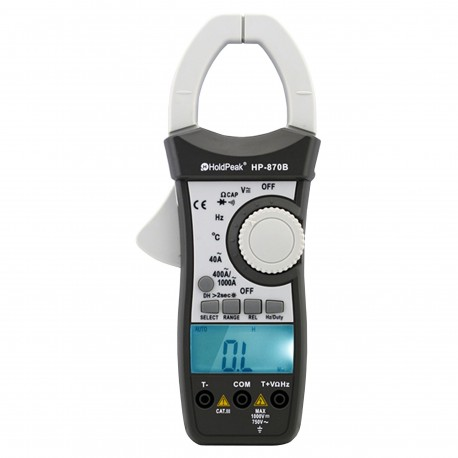
\includegraphics[scale=0.27]{amperimetro.jpg}
\caption{Amperímetro}
\end{center}
\end{figure}
\item \textbf{Voltímetro.} Mide el valor de la tensión en la corriente eléctrica, teniendo como unidad de medición el voltio. Es muy similar al galvanómetro, pero con la diferencia de que cuenta con una resistencia en serie.
\begin{figure}[H]
\begin{center}
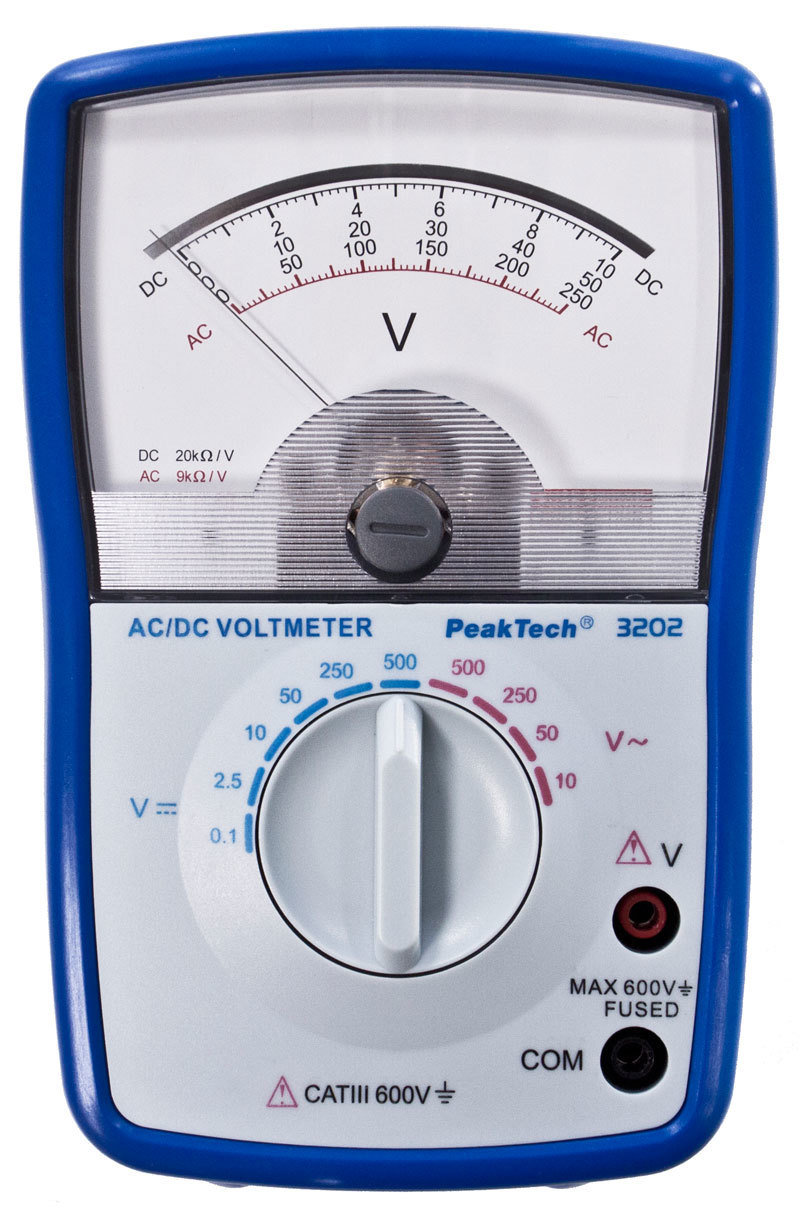
\includegraphics[scale=0.08]{voltimetro.jpg}
\caption{Voltímetro}
\end{center}
\end{figure}
\item \textbf{Multímetro.} Es un instrumento que emplea en su funcionamiento los parámetros del amperímetro, el voltímetro y el Ohmímetro. A través de una conmutador pueden ser seleccionadas sus funciones, dependiendo el tipo de corriente. Existen del tipo analógico y digital.
\begin{figure}[H]
\begin{center}
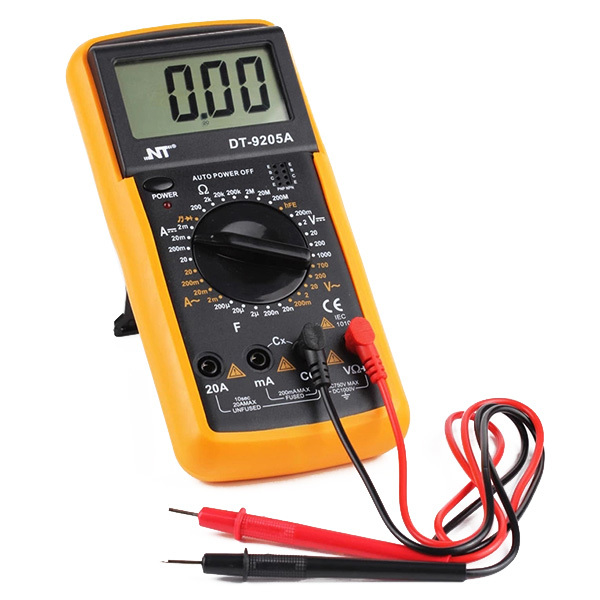
\includegraphics[scale=0.35]{multimetro.jpg}
\caption{Multímetro}
\end{center}
\end{figure}
\item \textbf{Osciloscopio.} Es un instrumento capaz de presentarnos sus resultados a través de representaciones gráficas, cuyas señales eléctricas pueden alterarse en el tiempo. Nos facilita visualizar eventos inusuales y transitorios además de ondas en circuitos eléctricos y electrónicos; y gracias a su análisis se puede detectar los problemas del funcionamiento de un determinado circuito.
\begin{figure}[H]
\begin{center}
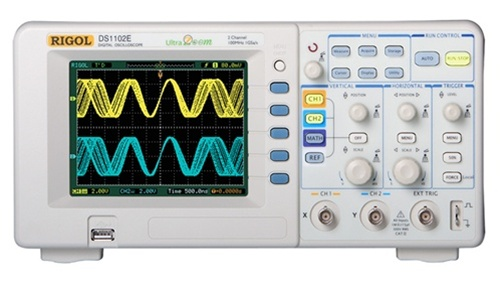
\includegraphics[scale=0.6]{osciloscopio.jpg}
\caption{Osciloscopio}
\end{center}
\end{figure}
\newpage
\item \textbf{Fuente de voltaje de corriente directa.} Fuente de poder de laboratorio típica. Se usan en escuelas y centros de investigación para alimentar circuitos electrónicos bajo prueba. Este modelo proporciona 3 salidas independientes con rangos de 0-30 volts y 0-3 amperes, y una salida fija de 5 volts con una corriente de 0-3 A. Estas fuentes son muy flexibles ya que las salidas variables se pueden configurar en modo serie o paralelo para obtener el doble de voltaje o corriente en la salida.
\begin{figure}[H]
\begin{center}
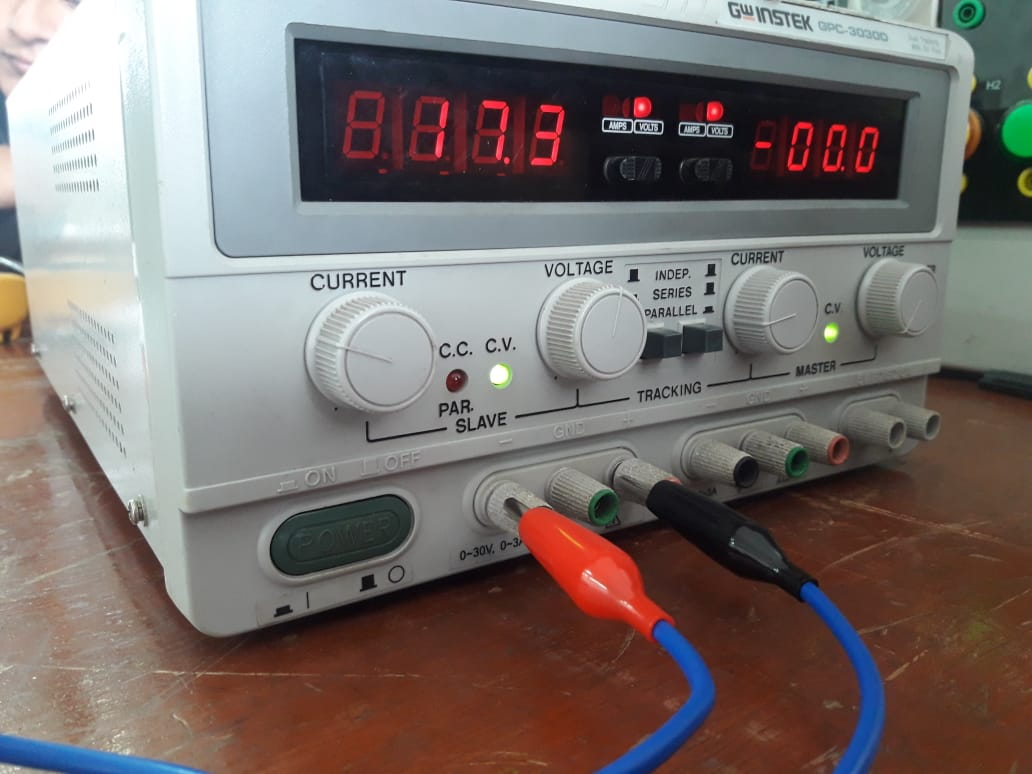
\includegraphics[height = 6cm, width =10.5cm]{fuentecd.jpeg}
\caption{Fuente de corriente directa}
\end{center}
\end{figure}
\item \textbf{Panel resistivo.}
\begin{figure}[H]
\begin{center}
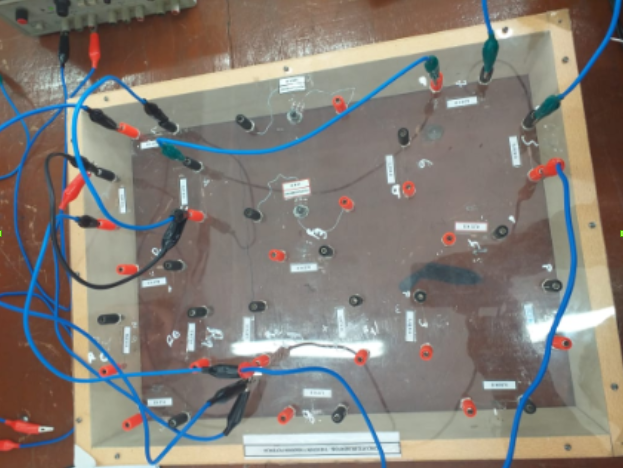
\includegraphics[height = 7.5cm, width =9cm, angle=90]{panelresistivo.png}
\caption{Panel resistivo}
\end{center}
\end{figure}
\item \textbf{Cables de conexión.}
\begin{figure}[H]
\begin{center}
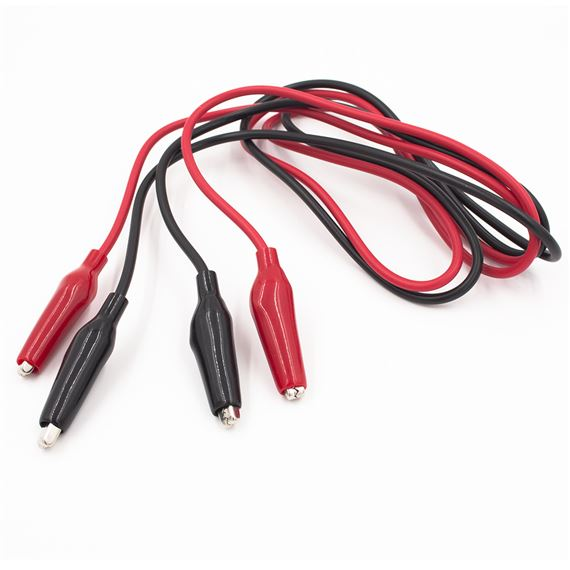
\includegraphics[height = 8cm, width =10.5cm]{cablesdeconexion.jpeg}
\caption{Cables de conexión - Cocodrilos}
\end{center}
\end{figure}
\end{enumerate}
%\part{Procedimiento}
\chapter{Uso de multímetro}
%El aparato cuenta con dos terminales cuyas polaridades se caracterizan por colores: Negro (-) y Rojo (+). Pudiendo encontrar 4 tipos de mediciones:
%\begin{enumerate}
%\item AC V.
%\item DC V.
%\item DC A.
%\item Ohmios.
%\end{enumerate}
\section{Resistencia}
\begin{enumerate}
\item Colocar el selector en posición “Ohm” o “Resistencia”. Cuando el multímetro mide la resistencia en ohmios, no podrá medir la continuidad, ya que la resistencia o continuidad son opuestas. Cuando hay poca resistencia, habrá mayor continuidad y viceversa. Inspeccionar en el dial para encontrar la escala de ohmios.
\item Observar el indicador de medida. Si las puntas de prueba no están en contacto con nada, la aguja o puntero de un multímetro analógico no se moverá de la posición de reposo más a la izquierda. Esto representa una cantidad infinita de resistencia o un “circuito abierto”.
\item Conectar la punta de prueba negra al borne marcado como (-). Luego, conecta la punta de prueba roja al borne marcado con el signo de la omega (símbolo del ohmio) o letra (R) cercana.
\item Medir la resistencia sobre un objeto funcional.
\end{enumerate}
\section{Voltaje}
\begin{enumerate}
\item Coloca el selector del multímetro en su rango más alto para voltios en corriente alterna (AC). Muchas veces se desconoce el voltaje del circuito a medir. Por este motivo, se deberá seleccionar el rango más alto posible para que los circuitos y el movimiento del aparato no se dañen por un voltaje mayor del esperado.
\item Conectar las puntas de prueba.
\item Ubicar las escalas de voltaje. Podría haber varias con diferentes valores máximos. El rango escogido en el selector determinará qué escala de voltaje leer.
\end{enumerate}
\section{Amperios}
\begin{enumerate}
\item Asegúrate de haber medido primero el voltaje. Necesitas determinar si el circuito es de corriente continua (DC) o alterna (AC) midiendo su voltaje como se ha explicado anteriormente.
\item Configura el multímetro en el rango más alto de amperios AC o DC que tenga.
\item  Medir la corriente sobre un objeto funcional.
\end{enumerate}
\newpage
\chapter{Código de colores}
\begin{figure}[H]
\begin{center}
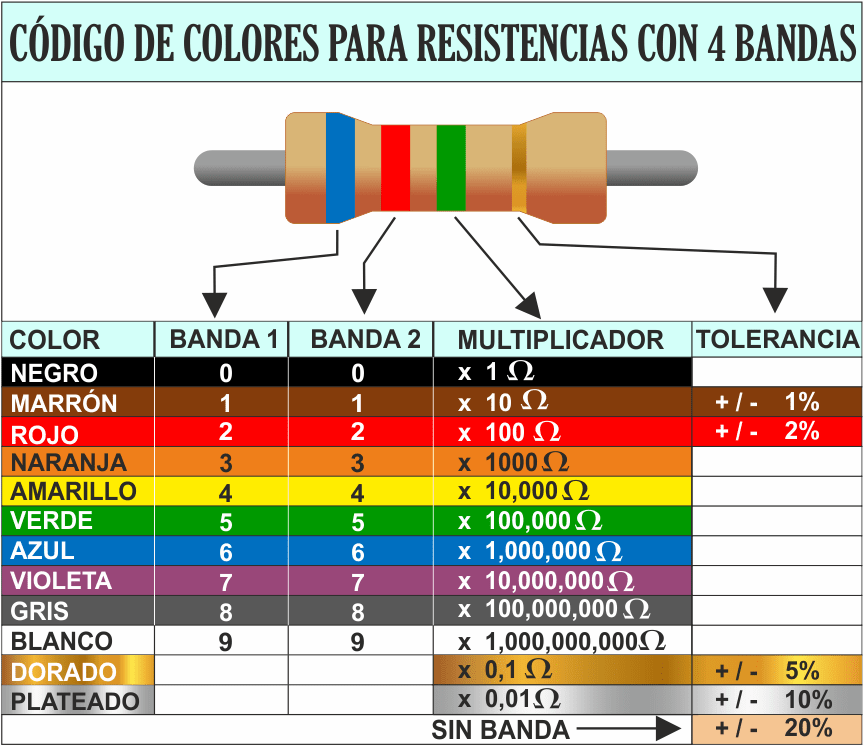
\includegraphics[scale=0.45]{resis5.png}
\caption{Código de colores resistencia 4 bandas}
\end{center}
\end{figure}
\begin{figure}[H]
\begin{center}
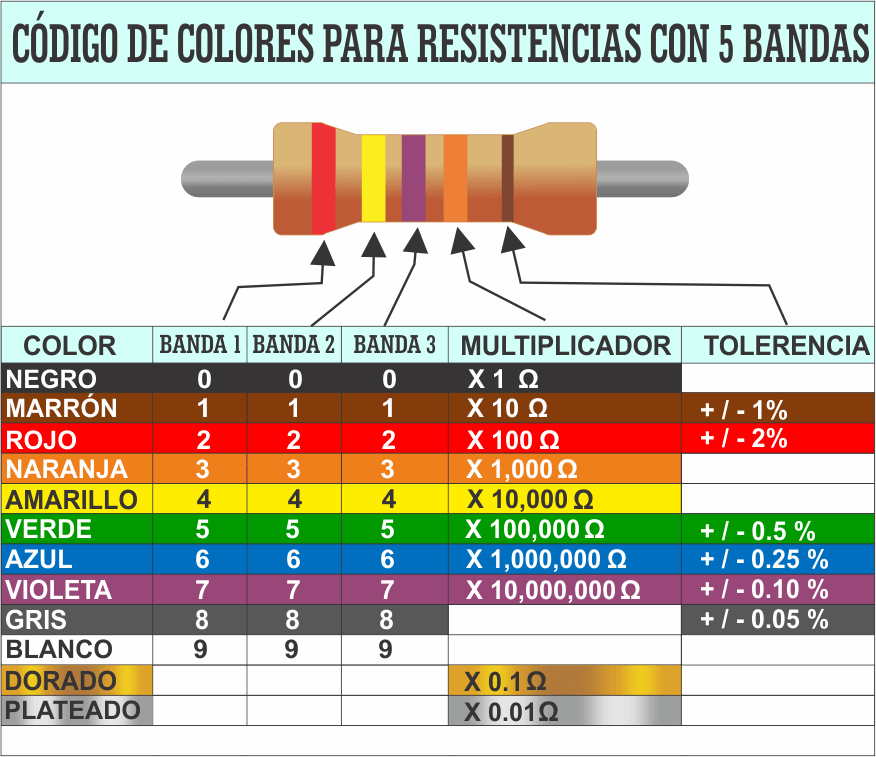
\includegraphics[scale=0.45]{resis4.png}
\caption{Código de colores resistencia 5 bandas}
\end{center}
\end{figure}
%\part{Procedimiento}
\part{Cuestionario}
\begin{enumerate}
\item \textbf{Hacer un diagrama del circuito usado en una hoja completa, indicando sentido de corrientes y polaridad de voltajes, así como los valores de las resistencias usadas.}\\
\textbf{Circuito 1}
\begin{figure}[H]
\centering
\begin{tikzpicture}[draw=DeepSkyBlue4,thin]
\tkzDefPoints{	0/0/A,
0/5/B,
6/5/C,
6/0/D,
9/5/E,
12/5/F,
12/0/G,
13/-0.5/H}
\draw[draw opacity=0, fill=yellow!30] (0,2.5) circle (.4);
\draw (C) to[R = 369.1\si{\ohm},color=Aquamarine4] (B) to[V=10V,color=red,thin] (A);
\draw (C) to[R = 361.9\si{\ohm},color=Aquamarine4] (D);
\draw (A) to (D);
\draw (D) to (G);
\draw (C) to[R = 501\si{\ohm},color=Aquamarine4] (E);
\draw (E) to[R = 271.2\si{\ohm},color=Aquamarine4] (F);
\draw (F) to[R = 193.3\si{\ohm},color=Aquamarine4] (G);
\draw (G) to ({13,0});
\draw ({13,0}) to (H) node[sground]{};
\end{tikzpicture}
\end{figure}
Resultado experimental
\begin{figure}[H]
\centering
\begin{tikzpicture}[draw=DeepSkyBlue4,thin]
\tkzDefPoints{	0/0/A,
0/5/B,
6/5/C,
6/0/D,
9/5/E,
12/5/F,
12/0/G,
13/-0.5/H}
\draw[draw opacity=0, fill=yellow!30] (0,2.5) circle (.4);
\draw (C) to[R = 369.1\si{\ohm},color=Aquamarine4] (B) to[V=10V,color=red,thin] (A);
\draw (C) to[R = 361.9\si{\ohm},color=Aquamarine4] (D);
\draw (A) to (D);
\draw (D) to (G);
\draw (C) to[R = 501\si{\ohm},color=Aquamarine4] (E);
\draw (E) to[R = 271.2\si{\ohm},color=Aquamarine4] (F);
\draw (F) to[R = 193.3\si{\ohm},color=Aquamarine4] (G);
\draw (G) to ({13,0});
\draw ({13,0}) to (H) node[sground]{};
\tkzLabelPoint[above](3,5.5){10.02V}
\tkzLabelPoint[above](2.2,5){-}
\tkzLabelPoint[above](3.8,5){+}
\tkzLabelPoint[above](5,2.3){10.01V}
\tkzLabelPoint[above](5.5,2.8){+}
\tkzLabelPoint[above](5.5,1.8){-}
\tkzLabelPoint[above](7.5,4){6.45V}
\tkzLabelPoint[above](6.7,4.5){+}
\tkzLabelPoint[above](8.3,4.5){-}
\tkzLabelPoint[above](10.5,4){2.152V}
\tkzLabelPoint[above](9.7,4.5){+}
\tkzLabelPoint[above](11.3,4.5){-}
\tkzLabelPoint[above](10.8,2.2){1.428V}
\tkzLabelPoint[above](11.5,2.8){+}
\tkzLabelPoint[above](11.5,1.8){-}
\end{tikzpicture}
\end{figure}
\newpage
Notamos que existe una gran diferencia entre los valores obtenidos. Esto se debe a que el circuito fue mal conectado; siendo los datos del laboratorio correspondientes a este otro circuito:
\begin{figure}[H]
\centering
\begin{tikzpicture}[draw=DeepSkyBlue4,thin]
\tkzDefPoints{	0/0/A,
0/5/B,
8/5/C,
8/0/D,
12.5/5/E,
16/5/F,
16/0/G,
16.5/-0.5/H,
5/3.5/I,
5/1.5/J,
10.5/3.5/K,
10.5/1.5/L,
9.5/5/M,
11/5/N,
13.5/5/O,
15/5/P,
15/3.5/R,
15/1.5/S,
3/5/T,
3/0/U}
\draw[draw opacity=0, fill=yellow!30] (0,2.5) circle (.4);
\draw (C) to (B) to[V=10V,color=red,thin] (A);
%\draw (B) to[V=\(100\si{\volt}\),color=red,thin] (A) to[R=\(1\si{\ohm}\),color=Aquamarine4] (C);				
%\draw (J) to[R=\(2\si{\ohm}\)] (C);
\draw (C) to[R = 361.9\si{\ohm},color=Aquamarine4] (D);
\draw (T) to[R = 100\si{\ohm},color=Aquamarine4] (U);
\draw (A) to (D);
\draw (D) to (G);
\draw (C) to[R = 501\si{\ohm},color=Aquamarine4] (E);
\draw (E) to[R = 271.2\si{\ohm},color=Aquamarine4] (F);
\draw (F) to[R = 193.3\si{\ohm},color=Aquamarine4] (G);
\draw (G) to ({16.5,0});
\draw ({16.5,0}) to (H) node[sground]{};
\draw (I) to ({3,3.5});
\draw (J) to ({3,1.5});
\draw (J) to[voltmeter] (I);
\draw (K) to ({8,3.5});
\draw (L) to ({8,1.5});
\draw (L) to[voltmeter] (K);
\draw (M) to ({9.5,6.5});
\draw (N) to ({11,6.5});
\draw ({9.5,6.5}) to[voltmeter] ({11,6.5});
\draw (O) to ({13.5,6.5});
\draw (P) to ({15,6.5});
\draw ({13.5,6.5}) to[voltmeter] ({15,6.5});
\draw (R) to ({16,3.5});
\draw (S) to ({16,1.5});
\draw (S) to[voltmeter] (R);
%\draw (D) to (G);
%\draw[rotate=0] (D) to[ammeter](3,1.5) to[european resistor = Z] (L);
%\draw[rotate=0] (G) to[voltmeter] (O);
%\draw (O) to (H);
%\draw (5.5,2.5) to[cute inductor=100\text{m}\si{\henry}] (5.5,0);
%\draw (C) to[short,-o] (D) to[open, -o] (E) to[cute inductor=2.5\si{\henry}] (F) to (G); %to[R=\(10\si{\ohm}\), v<=\(v_R\)] (G);
%\draw (A) to[color=Aquamarine4] (P);
%\draw (P) to (H);% to (G);% to[V=\(10\si{\volt}\)] (G);
%\draw (I) to[C=\(\frac{1}{40}\si{\farad}\), v<=\(v\)] (K) to (D);

%\draw[->, red, thick, >=stealth]([shift=(60:.4)]N) to[bend right=60] ([shift=(210:.4)]N);

%\draw[->, blue, thick, >=stealth]([shift=(220:.4)]S) to[bend left=60] ([shift=(60:.4)]S);

%\draw[->, blue, thick, >=stealth]([shift=(220:.4)]T) to[bend left=60] ([shift=(60:.4)]T);

\tkzLabelPoint[above](6.3,2.25){10V}
\tkzLabelPoint[above](11.7,2.3){10V}
\tkzLabelPoint[above](10.5,7){5.189V}
\tkzLabelPoint[above](14.2,7){2.809V}
\tkzLabelPoint[above](13.7,2.2){2.002V}
%\tkzLabelPoint[above](4.5,1.4){\(i_{2}\)}
\end{tikzpicture}
\end{figure}
Se observa, que los valores medidos en el laboratorio son muy cercanos a los obtenidos analíticamente.
\newpage
\textbf{Circuito 2}
\begin{figure}[H]
\begin{center}
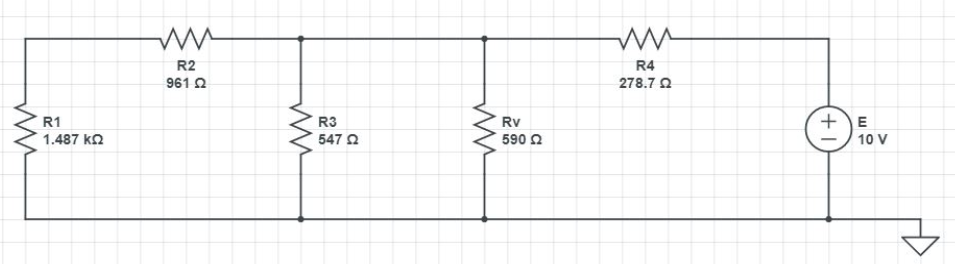
\includegraphics[scale=0.5]{circ2kesken.png}
\end{center}
\end{figure}
Resultado experimental
\begin{figure}[H]
\begin{center}
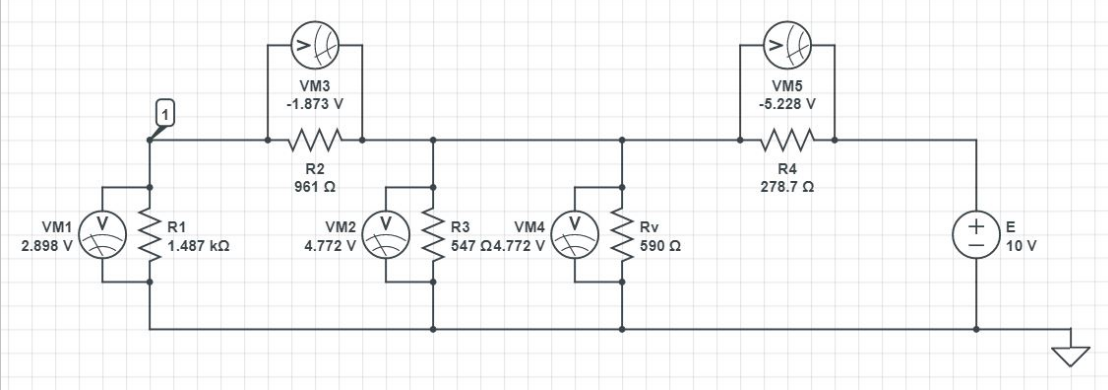
\includegraphics[scale=0.43]{circ2,1kesken.png}
\end{center}
\end{figure}
\newpage
\textbf{Circuito 3}
\begin{figure}[H]
\begin{center}
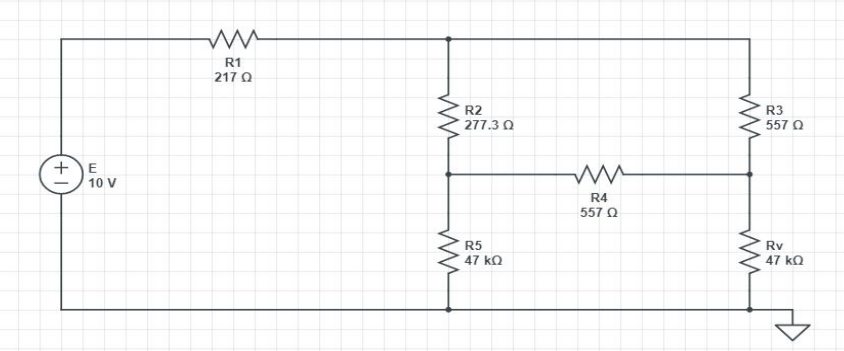
\includegraphics[scale=0.45]{circ3,1kesken.png}
\end{center}
\end{figure}
Resultado experimental
\begin{figure}[H]
\begin{center}
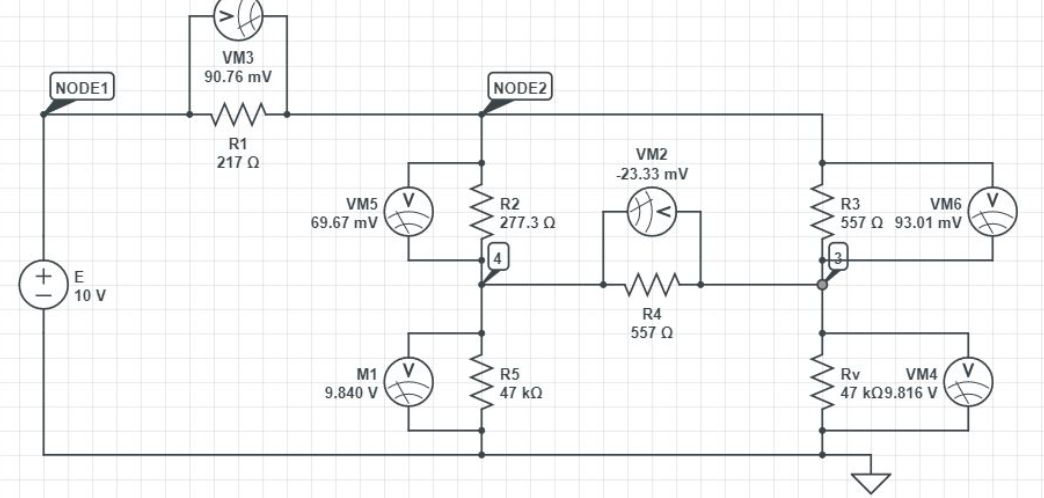
\includegraphics[scale=0.4]{circ3,2kesken.png}
\end{center}
\end{figure}
\newpage
\item \textbf{Con los valores medidos de tensión, comprobar la ley de Voltajes en cada malla, indicando el error experimental.}\\
\textbf{Circuito 1}\\
Resultado analítico
\begin{figure}[H]
\centering
\begin{tikzpicture}[draw=DeepSkyBlue4,thin]
\tkzDefPoints{	0/0/A,
0/5/B,
8/5/C,
8/0/D,
12.5/5/E,
16/5/F,
16/0/G,
16.5/-0.5/H,
3/5/I,
5/5/J,
6.8/3.5/K,
6.8/1.5/L,
9.5/5/M,
11/5/N,
13.5/5/O,
15/5/P,
15/3.5/R,
15/1.5/S,
4.4/1.7/T}
\draw[draw opacity=0, fill=yellow!30] (0,2.5) circle (.4);
\draw (C) to[R = 369.1\si{\ohm},color=Aquamarine4] (B) to[V=10V,color=red,thin] (A);
%\draw (B) to[V=\(100\si{\volt}\),color=red,thin] (A) to[R=\(1\si{\ohm}\),color=Aquamarine4] (C);				
%\draw (J) to[R=\(2\si{\ohm}\)] (C);
\draw (C) to[R = 361.9\si{\ohm},color=Aquamarine4] (D);
\draw (A) to (D);
\draw (D) to (G);
\draw (C) to[R = 501\si{\ohm},color=Aquamarine4] (E);
\draw (E) to[R = 271.2\si{\ohm},color=Aquamarine4] (F);
\draw (F) to[R = 193.3\si{\ohm},color=Aquamarine4] (G);
\draw (G) to ({16.5,0});
\draw ({16.5,0}) to (H) node[sground]{};
\draw (I) to ({3,6});
\draw (J) to ({5,6});
\draw ({3,6}) to[voltmeter] ({5,6});
\draw (K) to ({8,3.5});
\draw (L) to ({8,1.5});
\draw (L) to[voltmeter] (K);
\draw (M) to ({9.5,6.5});
\draw (N) to ({11,6.5});
\draw ({9.5,6.5}) to[voltmeter] ({11,6.5});
\draw (O) to ({13.5,6.5});
\draw (P) to ({15,6.5});
\draw ({13.5,6.5}) to[voltmeter] ({15,6.5});
\draw (R) to ({16,3.5});
\draw (S) to ({16,1.5});
\draw (S) to[voltmeter] (R);
%\draw (D) to (G);
%\draw[rotate=0] (D) to[ammeter](3,1.5) to[european resistor = Z] (L);
%\draw[rotate=0] (G) to[voltmeter] (O);
%\draw (O) to (H);
%\draw (5.5,2.5) to[cute inductor=100\text{m}\si{\henry}] (5.5,0);
%\draw (C) to[short,-o] (D) to[open, -o] (E) to[cute inductor=2.5\si{\henry}] (F) to (G); %to[R=\(10\si{\ohm}\), v<=\(v_R\)] (G);
%\draw (A) to[color=Aquamarine4] (P);
%\draw (P) to (H);% to (G);% to[V=\(10\si{\volt}\)] (G);
%\draw (I) to[C=\(\frac{1}{40}\si{\farad}\), v<=\(v\)] (K) to (D);

%\draw[->, red, thick, >=stealth]([shift=(60:.4)]N) to[bend right=60] ([shift=(210:.4)]N);

%\draw[->, blue, thick, >=stealth]([shift=(220:.4)]S) to[bend left=60] ([shift=(60:.4)]S);

%\draw[->, blue, thick, >=stealth]([shift=(220:.4)]T) to[bend left=60] ([shift=(60:.4)]T);

\tkzLabelPoint[above](4,6.5){-5.837V}
\tkzLabelPoint[above](5.6,2.3){4.163V}
\tkzLabelPoint[above](10.5,7){-2.16V}
\tkzLabelPoint[above](14.2,7){-1.169V}
\tkzLabelPoint[above](13.6,2.2){833.4 mV}
%\tkzLabelPoint[above](4.5,1.4){\(i_{2}\)}
\end{tikzpicture}
\end{figure}
\textbf{Circuito 2}\\
Resultado analítico
\begin{figure}[H]
\begin{center}
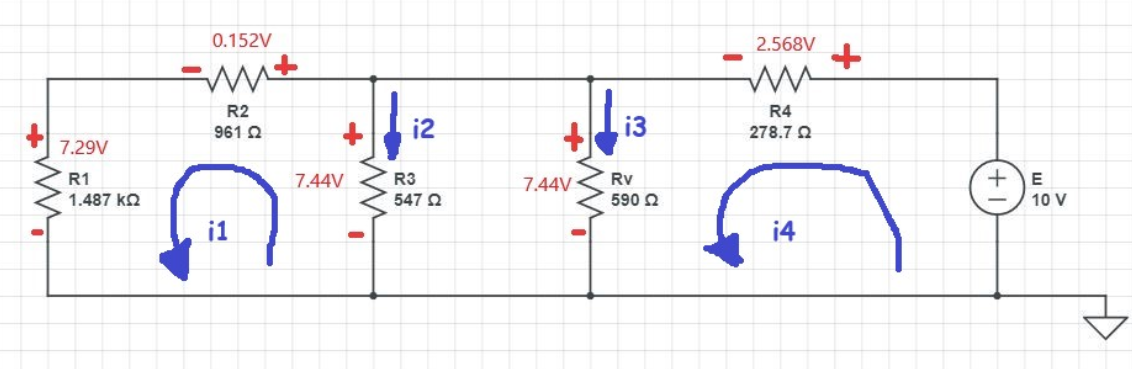
\includegraphics[width=17cm, height=8cm]{circ2,2kesken.png}
\end{center}
\end{figure}
\newpage
\textbf{Circuito 3}\\
Resultado analítico
\begin{figure}[H]
\begin{center}
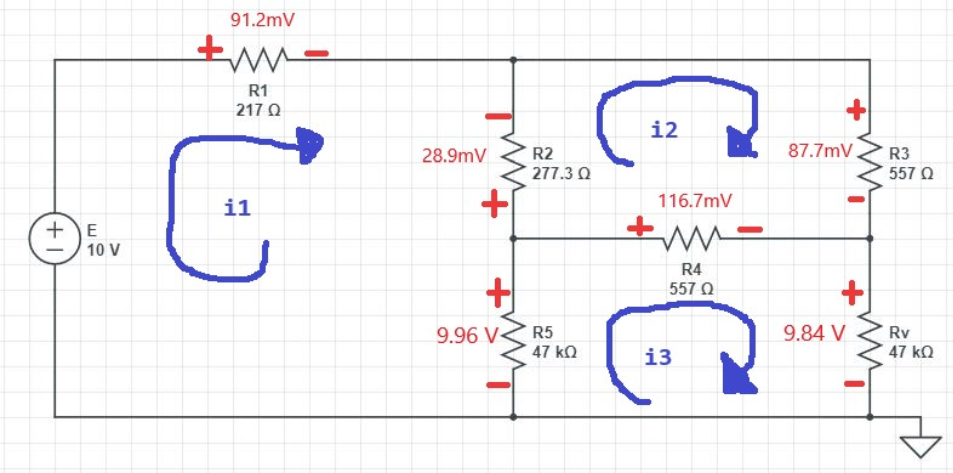
\includegraphics[scale=0.45]{circ3,3kesken.png}
\end{center}
\end{figure}
\item \textbf{Verificar de igual forma la Ley de las Corrientes en cada nodo, haciendo notar el error de las mediciones.}\\
\textbf{Circuito 1}\\
\begin{figure}[H]
\begin{center}
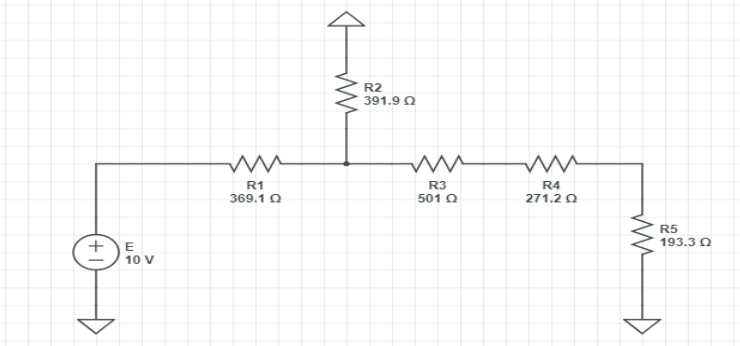
\includegraphics[scale=0.52]{sergodcirc1,1.png}
\end{center}
\end{figure}
Transformamos el circuito a una forma equivalente para unir las 3 líneas a tierra.
\begin{figure}[H]
\begin{center}
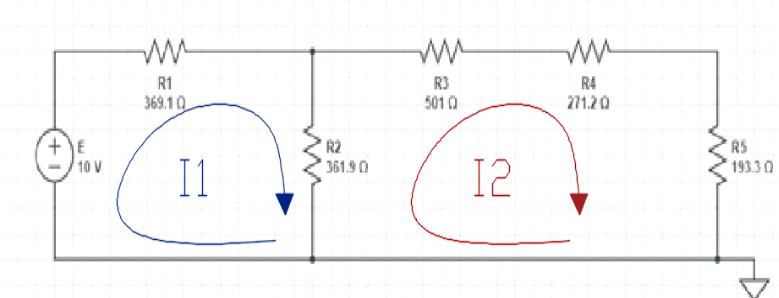
\includegraphics[scale=0.6]{sergodcirc1,2.png}
\end{center}
\end{figure}
Aplicamos la segunda ley de Kircchoff:\\
Malla 1: $10 = 731I_{1} - 361.9I_{2}$\\
Malla 2: $0 = -361.9I_{1} + 1327.4I_{2}$\\
De forma matricial:
$$
\begin{bmatrix}
10\\
0
\end{bmatrix}
 = 
\begin{bmatrix}
731 & -361.9\\
-361.9 & 1327.4
\end{bmatrix} \cdot \begin{bmatrix}
I_{1}\\
I_{2}
\end{bmatrix}
$$
Resolviendo:
$$
I_{1} = 15.8144\,\mathrm{mA} \hspace{30pt} I_{2} = 4.31163\,\mathrm{mA}
$$
\begin{figure}[H]
\begin{center}
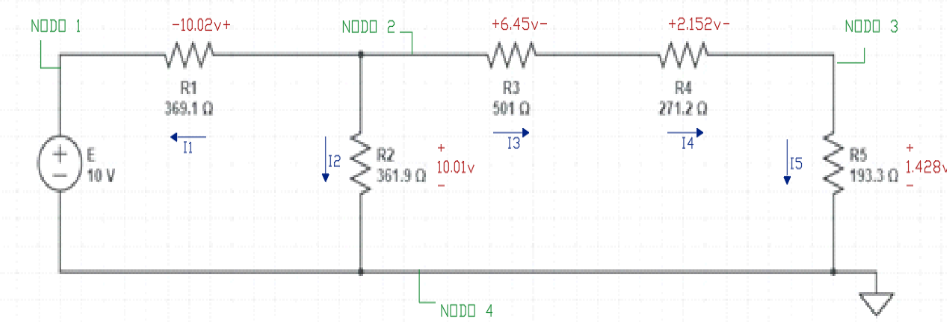
\includegraphics[scale=0.5]{sergodcirc1,3.png}
\end{center}
\end{figure}
Aplicamos la ley de ohm para hallar las corrientes experimentales ($V = I \cdot R$):
$$
I_{1} = 27.1471\,\mathrm{mA} \hspace{15pt} I_{2} = 27.6595\,\mathrm{mA} \hspace{15pt} I_{3}=12.8842\,\mathrm{mA} \hspace{15pt} I_{4} = 7.8613\,\mathrm{mA} \hspace{15pt} I_{5} = 7.3875\,\mathrm{mA}
$$
Aplicamos la primera ley de Kirchhoff para cada nodo:
$$
\sum_{k=1}^{n} I_{k} = 0
$$
Nodo 2: $\vert -I_{1} - I_{2} - I_{3} \vert  = 67.6908\,\mathrm{mA}$\\
Nodo 3: $\vert I_{4} - I_{5} \vert  = 0.47382\,\mathrm{mA}$\\
Nodo 4: $\vert I_{1} + I_{2} + I_{5} \vert  = 62.19408\,\mathrm{mA}$\\
\textbf{Circuito 2}\\
\begin{figure}[H]
\begin{center}
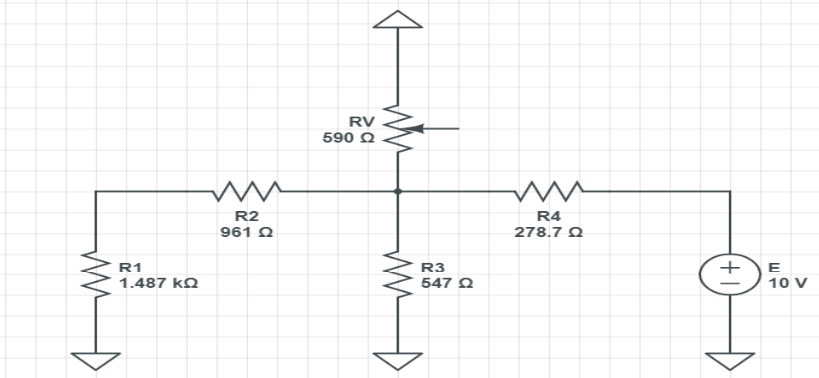
\includegraphics[scale=0.55]{sergodcirc2,1.png}
\end{center}
\end{figure}
Transformamos el circuito.
\begin{figure}[H]
\begin{center}
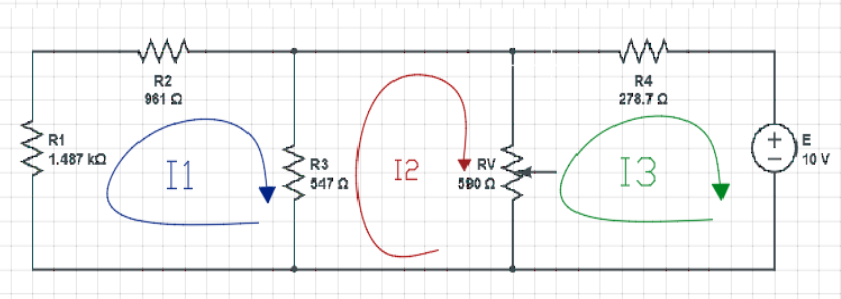
\includegraphics[scale=0.55]{sergodcirc2,2.png}
\end{center}
\end{figure}
Aplicamos la segunda ley de Kircchoff:\\
Malla 1: $0 = 2995I_{1} - 547I_{2}$\\
Malla 2: $0 = -547I_{1} + 1137I_{2} - 590I_{3}$\\
Malla 3: $-10 = -590I_{2} + 868.7I_{3}$\\
De forma matricial:
$$
\begin{bmatrix}
0\\
0\\
-10
\end{bmatrix}
 = 
\begin{bmatrix}
2995 & -547 & 0\\
-547 & 1137 & -590\\
0 & -590 & 868.7
\end{bmatrix} \cdot \begin{bmatrix}
I_{1}\\
I_{2}\\
I_{3}
\end{bmatrix}
$$
Resolviendo:
$$
I_{1} = 15.8144\,\mathrm{mA} \hspace{30pt} I_{2} = 4.31163\,\mathrm{mA} \hspace{30pt} I_{3} = -18.76\,\mathrm{mA}
$$
\begin{figure}[H]
\begin{center}
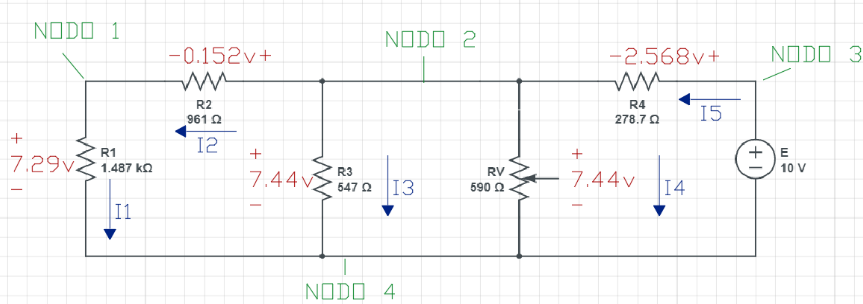
\includegraphics[scale=0.45]{sergodcirc2,3.png}
\end{center}
\end{figure}
Aplicamos la ley de ohm para hallar las corrientes experimentales ($V = I \cdot R$):
$$
I_{1} = 4.9025\,\mathrm{mA} \hspace{15pt} I_{2} = 0.1587\,\mathrm{mA} \hspace{15pt} I_{3}=13.6015\,\mathrm{mA} \hspace{15pt} I_{4} = 12.61026\,\mathrm{mA} \hspace{15pt} I_{5} = 9.2142\,\mathrm{mA}
$$
Aplicamos la primera ley de Kirchhoff para cada nodo:\\
Nodo 1: $\vert I_{2} - I_{1} \vert  = 4.7438\,\mathrm{mA}$\\
Nodo 2: $\vert I_{5} - I_{2} - I_{3} - I_{4} \vert  = 17.1562\,\mathrm{mA}$\\
Nodo 4: $\vert I_{1} + I_{3} + I_{4} - I_{5} \vert  = 21.9\,\mathrm{mA}$\\
\textbf{Circuito 3}\\
\begin{figure}[H]
\begin{center}
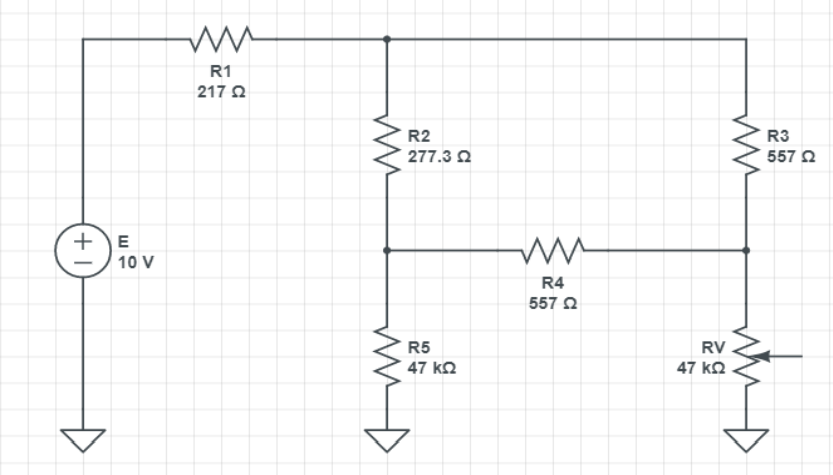
\includegraphics[scale=0.45]{sergodcirc3,2.png}
\end{center}
\end{figure}
Transformamos el circuito.
\begin{figure}[H]
\begin{center}
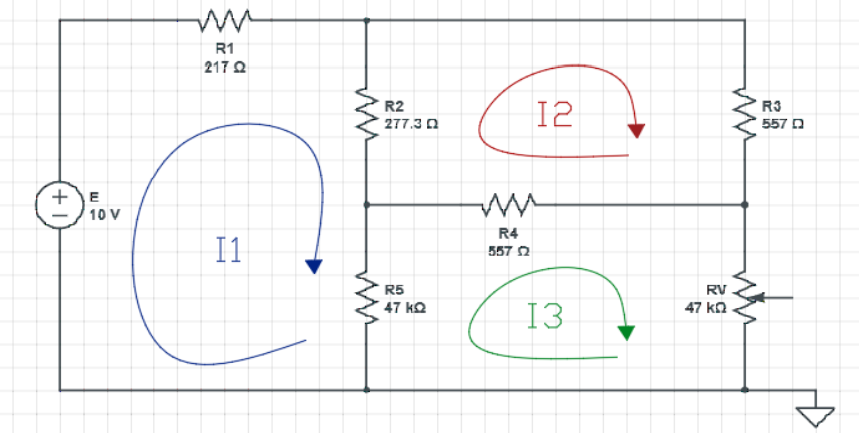
\includegraphics[scale=0.45]{sergodcirc3,3.png}
\end{center}
\end{figure}
Aplicamos la segunda ley de Kircchoff:\\
Malla 1: $10 = 47494.3I_{1} - 277.3I_{2} - 47000I_{3}$\\
Malla 2: $0 = -277.3I_{1} + 1391.3I_{2} - 557I_{3}$\\
Malla 3: $0 = -47000I_{1} - 557I_{2} + 94557I_{3}$\\
De forma matricial:
$$
\begin{bmatrix}
10\\
0\\
0
\end{bmatrix}
 = 
\begin{bmatrix}
47494.3 & -277.3 & -47000\\
-277.3 & 1391.3 & -557\\
-47000 & -557 & 94557
\end{bmatrix} \cdot \begin{bmatrix}
I_{1}\\
I_{2}\\
I_{3}
\end{bmatrix}
$$
Resolviendo:
$$
I_{1} = 0.41821\,\mathrm{mA} \hspace{30pt} I_{2} = 0.167\,\mathrm{mA} \hspace{30pt} I_{3} = 0.21\,\mathrm{mA}
$$
\begin{figure}[H]
\begin{center}
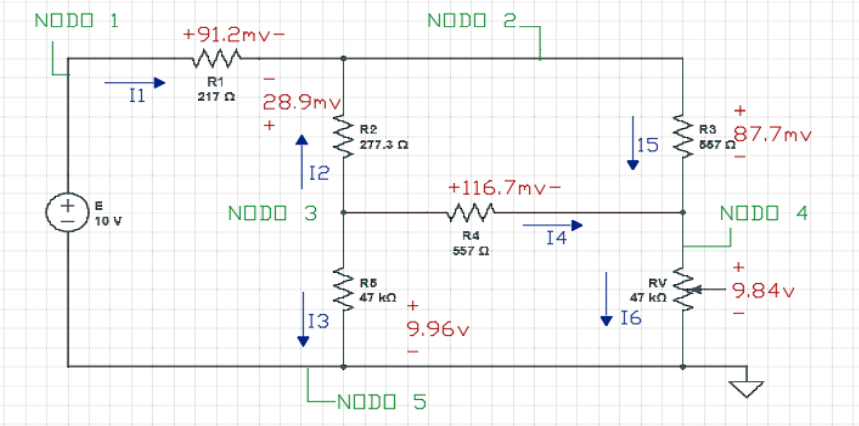
\includegraphics[scale=0.45]{sergodcirc3,1.png}
\end{center}
\end{figure}
Aplicamos la ley de ohm para hallar las corrientes experimentales ($V = I \cdot R$):
$$
I_{1} = 0.42\,\mathrm{mA} \hspace{12pt} I_{2} = 0.1042\,\mathrm{mA} \hspace{12pt} I_{3}=0.212\,\mathrm{mA} \hspace{12pt} I_{4} = 0.21\,\mathrm{mA} \hspace{12pt} I_{5} = 0.157\,\mathrm{mA} \hspace{12pt} I_{6} = 0.21\,\mathrm{mA}
$$
Aplicamos la primera ley de Kirchhoff para cada nodo:\\
Nodo 2: $\vert I_{1} + I_{2} - I_{5} \vert  = 0.367\,\mathrm{mA}$\\
Nodo 3: $\vert -I_{2} - I_{3} - I_{4} \vert  = 0.5256\,\mathrm{mA}$\\
Nodo 4: $\vert I_{4} + I_{5} - I_{6} \vert  = 0.15656\,\mathrm{mA}$\\
Nodo 5: $\vert I_{3} + I_{6} - I_{1} \vert  = 0.002034\,\mathrm{mA}$
\item \textbf{Explicar algunas justificaciones de los errores para los pasos anteriores.}\\
Los errores, sobre todo en el primer circuito, se deben a la pobre sujeción que se le dio a una resistencia, pues para medirla se tuvo que voltear el panel resistivo de costado, y medirla por abajo (alambre) para mayor exactitud, pero al realizar este movimiento se soltó levemente un cable que después pudimos verificarlo al no tomar en cuenta la resistencia sospechosa.\\
También la imprecisión del multímetro utilizado jugó un rol muy importante, posiblemente no tuvo una calibración o mantenimiento ideal, lo cual sumado a factores externos provocó alteraciones en ciertos valores reales de resistencias, por ejemplo, cuando medíamos una resistencia de 0.46k$\Omega$, el téster oscilaba erráticamente dando valores muy altos, se tenía que reiniciarlo para que de un valor cercano a 0.46k$\Omega$.\\
En este laboratorio no se contó con amperímetro pues el fusible de nuestro multímetro estaba dañando. También había algunas resistencias quemadas que no pudimos utilizar. Gran parte del error se podría deber también a la medición que hicimos de las resistencias, lo medimos por debajo del panel de resistencias para tener una calidad de datos, sin embargo, se debe tener en cuenta la resistencia de la zona soldada pues recordemos que ahí puede haber impurezas, incluso si no las hay al ser una zona de ensanchamiento hace que la resistencia del conductor aumente quitándole el privilegio de ``ideal''.\\
Sin duda alguna el desgaste de las herramientas de medición juega un papel importante en la lectura de datos de laboratorio, para el tercer circuito tuvimos que prender/apagar cada vez que medíamos un voltaje y luego resistencias, en ese momento aún no sabíamos si iba ser mejor hacer eso, solo probamos, pero al momento de desarrollar este informe llegamos a la conclusión de que el circuito tres fue el más exacto y con notorio bajo margen de error.
\newpage
\item \textbf{Con las resistencias medidas, solucionar el circuito en forma teórica indicando las tensiones y corrientes en cada elemento en un diagrama similar al punto 1.}\\
\textbf{Circuito 1}
\begin{figure}[H]
\begin{center}
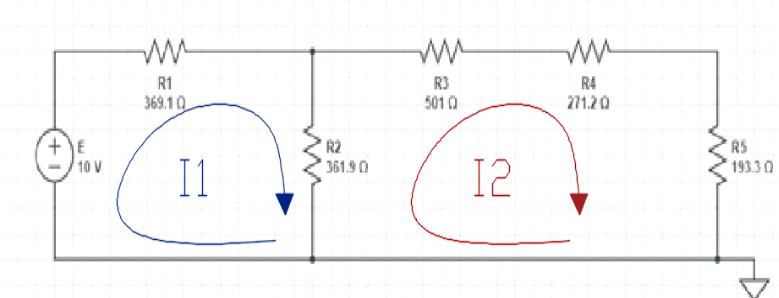
\includegraphics[scale=0.55]{sergodcirc1,2.png}
\end{center}
\end{figure}
El circuito nos queda:
\begin{figure}[H]
\begin{center}
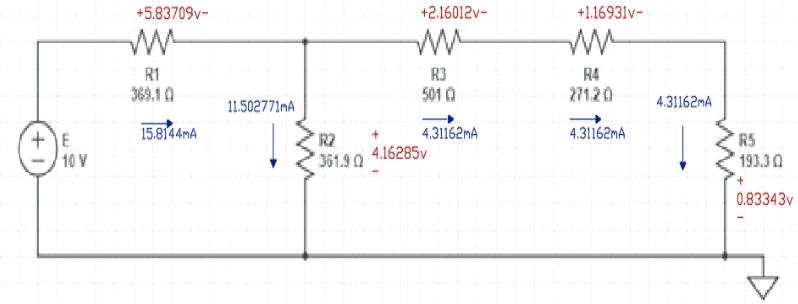
\includegraphics[scale=0.55]{sergodcirc5,1.png}
\end{center}
\end{figure}
\newpage
\textbf{Circuito 2}
\begin{figure}[H]
\begin{center}
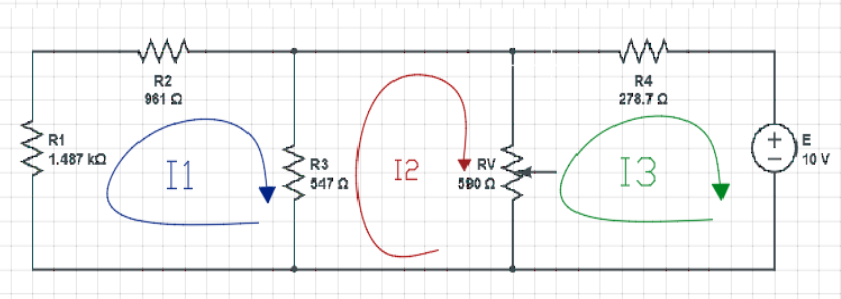
\includegraphics[scale=0.55]{sergodcirc2,2.png}
\end{center}
\end{figure}
$$
I_{1} = -1.9491\,\mathrm{mA} \hspace{20pt} I_{2} = -10.6724\,\mathrm{mA} \hspace{20pt} I_{3} = -18.76\,\mathrm{mA}
$$
El circuito nos queda:
\begin{figure}[H]
\begin{center}
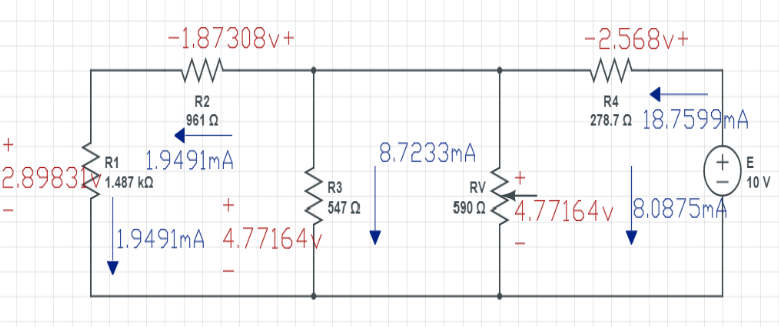
\includegraphics[scale=0.55]{sergodcirc5,2.png}
\end{center}
\end{figure}
\newpage
\textbf{Circuito 3}
\begin{figure}[H]
\begin{center}
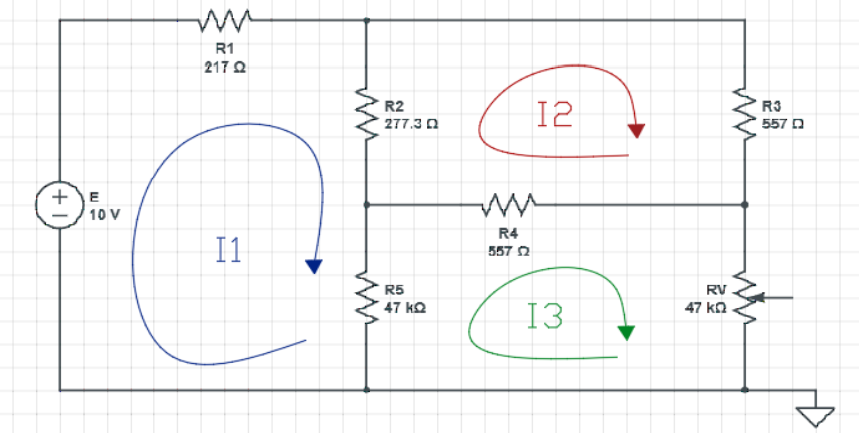
\includegraphics[scale=0.55]{sergodcirc3,3.png}
\end{center}
\end{figure}
$$
I_{1} = 0.41821\,\mathrm{mA} \hspace{20pt} I_{2} = 0.167\,\mathrm{mA} \hspace{20pt} I_{3} = 0.2088\,\mathrm{mA}
$$
El circuito nos queda:
\begin{figure}[H]
\begin{center}
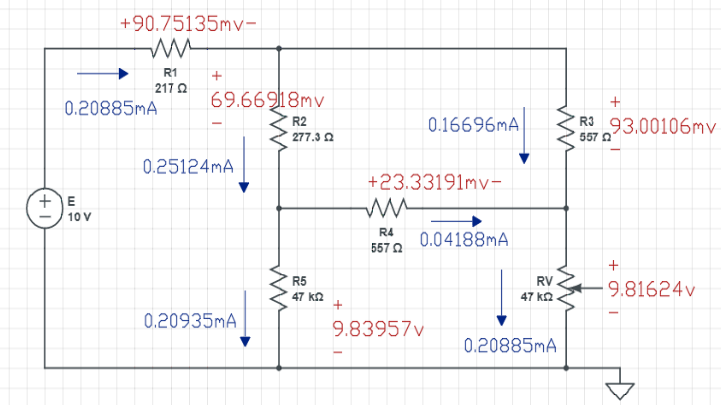
\includegraphics[scale=0.55]{sergodcirc5,3.png}
\end{center}
\end{figure}
\newpage
\item \textbf{Comparar los valores teóricos y experimentales, indicando el error absoluto y relativo porcentual, coméntelo}\\
De los datos obtenidos experimentalmente en el laboratorio se hizo la siguiente gráfica:
\begin{figure}[H]
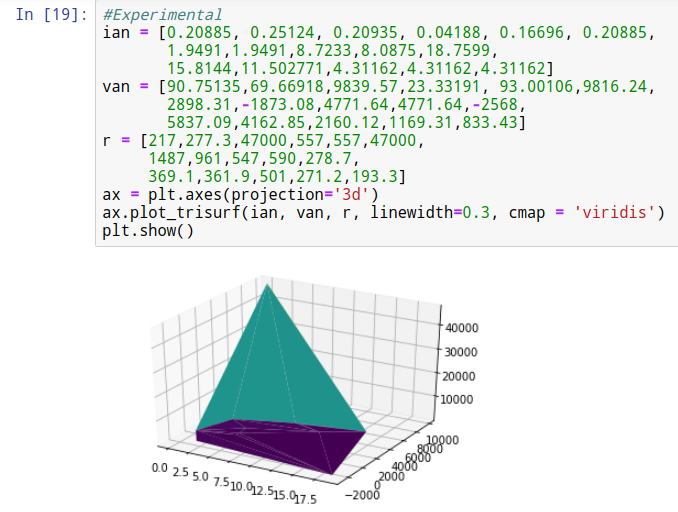
\includegraphics[scale=0.6]{experimentaldata.png}
\end{figure}
Mientras que con los datos analíticamente se obtuvo:
\begin{figure}[H]
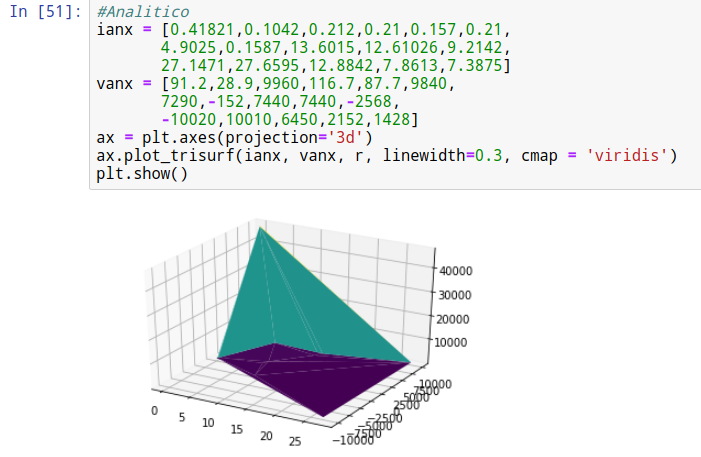
\includegraphics[scale=0.6]{analitico2.png}
\end{figure}
Se observa que ambas gráficas se asemejan. Para estimar el grado de error utilizamos como métrica los mínimos cuadrados:
\begin{figure}[H]
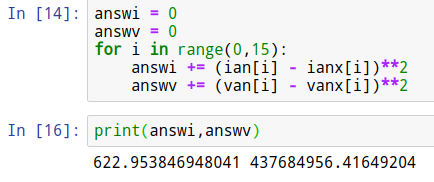
\includegraphics[scale=0.5]{errordata.png}
\end{figure}
Obtenemos como error para la corriente el valor de $622.9538469\,\mathrm{mA}^{2}$, mientras que para el voltaje el error es de $437684956.41649\,\mathrm{mV}^{2}$. Normalizando este error para unidades coherentes:
$$
\mathrm{Error \; \; I = 24.959\,\mathrm{mA}} \hspace{20pt} \mathrm{Error \; \; V = 20.92092\,\mathrm{V}}
$$
Para el error porcentual calculamos la diferencia relativa general:
\begin{figure}[H]
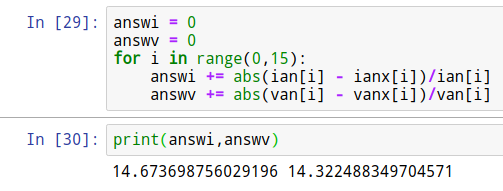
\includegraphics[scale=0.5]{errorporc.png}
\end{figure}
Consideramos la media del error como una métrica válida para el error porcentual relativo:
$$
\mathrm{Error \; \; I = \frac{\sqrt{14.6736987}}{15}\cdot 100\% = 25.5375\%} \hspace{20pt} \mathrm{Error \; \; V = \frac{\sqrt{14.322488349}}{15}\cdot 100\% = 25.23\%}
$$
Observamos que estos errores son muy grandes; esto es debido a que la conexión del primer circuito fue puesta en paralelo. La mayor parte del error sucede en el primer circuito. Como consideración debe tomarse especial atención para la conexión de los circuitos para obtener mejores resultados.
\item \textbf{Comentar sobre las posibles fuentes de error y observaciones sobre la experiencia realizada.}\\
Como se mencionó en la parte 4; los errores se deben en mayor medida a la mala sujeción de algunas resistencias en el tablero. Siendo los valores que se midieron solo voltajes; y con estos se halló las respectivas corrientes. La propagación del error se hace mayor al no tener un método directo de medición para la corriente.
\end{enumerate}
\part{Conclusiones y recomendaciones}
\chapter{Conclusiones}
\begin{enumerate}
\item Las leyes de Kirchhoff son muy útiles en la solución de circuitos eléctricos y facilitan su comprensión, la exactitud de estas leyes la comprobamos en el circuito numero tres en el cual tuvimos la pequeña consideración de reiniciar el multímetro cada vez que se hacía una medición.
\item Se recomienda, al conectar el multímetro en serie, no abusar de el voltaje pues eso seguramente va a quemar el fusible abriendo el circuito interno del multímetro, lo cual dificulta significativamente la tarea de próximos grupos de trabajo en el laboratorio que se ven afectados, esto lo pudimos comprobar el día de la experiencia pues con la intensidad de corriente experimental hubiésemos podido verificar muchas cosas.
\item Se recomienda verificar si las resistencias están en buen estado, recordemos que algunas se encuentran quemadas y al momento de hacer un circuito es tedioso darse cuenta de que una está mal y tal vez por la disposición del mismo no poder cambiarla.
\item Es recomendable utilizar valores cercanos de resistencias, es decir, tratar que estén en el mismo orden, para que la intensidad de corriente se vea menos afectada por la gran diferencia de resistencias y no tenga valores desbordantes en ciertas mallas o ramas e ínfimos en otras. 
\item Es necesario seguir las normas de seguridad del laboratorio para evitar accidentes.
\item Se comprobó la validez de las leyes de Kirchhoff.
\item Mantener limpio el laboratorio es importante para evitar entorpecer el trabajo.
\end{enumerate}

\begin{thebibliography}{99}  %%%este es un contador para el número de bibliografías utilizados.
\addcontentsline{toc}{chapter}{Bibliograf\'{\i}a} %%% Para introducir la bibliografía en el índice.
%\bibitem{Rahman}{Rahman,Aminur y Doe, Hidekazu; ``Ion transfer of tetraalkylammonium cations at an interface between 
%frozen aqueous solution and 1,2-dichloroethane".{\em{Journal of Electroanalytical Chemistry}} {\bfseries 424},159,(1997).}
\bibitem{Gro}{Boylestad, Robert M. ``Introducción al análisis de circuitos''. {\em{Pearson}}}
\bibitem{Gro}{Sadiku, Matthew N. ``Fundamemtos de circuitos eléctricos''. {\em{Mc Graw Hill}}}
%\bibitem{Ding}{Ding, Zhifeng. ``Spectroelectrochemistry and photoelectrochemistry of charge transfer at liquid/liquid
%interfaces". {\em {Tesis, EPFL,}}(1999).}
%\bibitem{AL}{Alonso, Jose M. \em{Técnicas de mecanizado 1}}
%\bibitem{AL}{Alonso, Jose M. ``Técnicas de mecanizado 1". {\em{Paraninfo}} {\bfseries España-Madrid}, 6-20, (2001).}
%\bibitem{Samec2}{Samec Z., Lhotsky A., Jänchenová H., y Marecek, V. ``Interfacial tension and impedance measurements
%of interfaces between two inmiscible electrolyte solutions". {\em{Journal of Electroanalytical Chemistry}} {\bfseries
%43}, 47, (2000).}
%\bibitem{Day}{Day R.A. y Underwood A.L. {\textit{Química Analítica Cuantitativa}},5ºed. Prentice-Hall, México, 1998. 45-48.}
%\bibitem{Keyser}{Farah Abud, Michel. ``Determinación de la vida útil en herramientales de corte endurecido por el proceso de borurización en pasta''. {\em{Instituto tecnológico y de estudios superiores de Monterrey}}}
%\bibitem{Zolotorevski}{Escalona, I. ``Máquinas: herramientas por arranque de viruta.''.{\em{El Cid Editor.}}}
%\bibitem{Lasheras}{Lasheras. ``Tecnología de los Materiales Industriales''.} 
%\bibitem{Dieter}{Dieter. ``Metalurgia mecánica''.}
%\bibitem{Apraiz}{Apraiz, J. ``Tratamiento Térmico de los Aceros''.}
%\bibitem{Smith}{Smith, William F. y Ph.D. Hashemi, Javad ``Ciencia e ingeniería de materiales". {\em{
%Madrid: McGraw-Hill, Interamericana de España.}} 570, (2004).} 
%\bibitem{Callister}{Callister, William D. y Rethwisch, David G. ``Introducción a la ingeniería de los materiales''. %{\em{Barcelona Reverté.}}, 960, (2007).} 
%\bibitem{Askeland}{Askeland, Donald R., Pradeep P. Phulé y Wright, Wendelin J. ``Ciencia e ingeniería de los materiales''.{\em{México, D.F. Internacional Thomson Editores.}} {\textit{$6^{ta}$ edición}}, 1004, (2012).}
%\bibitem{HARDBANDING}{Tabla de conversión de escala de durezas. \begin{verbatim}http://%hardbandingsolutions.com/postle_sp/hardness.php
%\end{verbatim}}
\bibitem{PR}{Von Below, Joachim. ``Kirchhoff laws and diffusion on networks''. \begin{verbatim}
https://core.ac.uk/download/pdf/82153964.pdf
\end{verbatim}}
%\bibitem{HE}{Fresadora. \begin{verbatim} http://lizdenbow.blogspot.com/
%\end{verbatim}}
%\bibitem{ASTM}{Normas ASTM.}
%\bibitem{NTP}{Normas NTP.}
\end{thebibliography}
\end{document}
